\documentclass{article}

\usepackage[utf8]{inputenc}
\usepackage{tabularx}
\usepackage{booktabs}
\usepackage{graphicx}
\usepackage[hidelinks]{hyperref}
\usepackage{geometry}
\usepackage{amsmath}
\geometry{a4paper, margin=1in}

\title{Early fault detection using Slope Entropy on embedded industrial systems}
\author{Jorge Peris Belenguer \\ Smart Technologies in Industry 4.0, MUCEIM}
\date{}

\begin{document}

\maketitle

\begin{abstract}
This paper presents an embedded implementation of early fault detection for industrial bearings using a novel non-linear complexity estimator called Slope Entropy. The methodology is evaluated using the NASA IMS Bearing Dataset. The pipeline includes data preprocessing, segmentation, and highly optimized vectorized feature extraction simulating edge computing constraints (e.g., Raspberry Pi). Our computational analysis demonstrates that the algorithm exhibits extreme efficiency, capturing dynamic degradation shifts well before catastrophic failures occur.
\end{abstract}

\textbf{Keywords:} Raspberry Pi, Python, IMS Bearings, Slope Entropy


\section{Introduction}
As the industrial landscape shifts toward Industry 4.0, predictive maintenance has emerged as a cornerstone for optimizing manufacturing efficiency and minimizing unexpected downtimes. Rolling element bearings are ubiquitous in rotating machinery, yet they remain one of the most frequent causes of mechanical breakdowns. Identifying localized defects in their early stages allows maintenance personnel to schedule repairs proactively, preventing catastrophic failures that disrupt production lines and incur severe economic losses.

Traditionally, industrial condition monitoring relies heavily on linear vibration analysis. Techniques such as the Fast Fourier Transform (FFT) and envelope analysis are extensively employed to extract characteristic fault frequencies from raw signals. However, rotating machinery operates in dynamic, noisy environments where vibrations often exhibit highly non-stationary and non-linear behaviors. As a result, classical frequency-domain approaches may struggle to identify weak incipient defect signatures masked by background friction noise and mechanical resonances.

To overcome the limitations of linear methods, non-linear time series analysis has gained significant traction. Entropy-based methods, which quantify the inherent complexity and predictability of dynamical systems, are particularly well-suited for machine condition monitoring. When a bearing is healthy, its vibration is characterized by random, high-complexity noise. Conversely, when a structural defect occurs, the rhythmic impacts of the rolling elements generate a more deterministic, structured, and periodic signal, leading to a measurable drop in entropy.

This study implements a novel complexity estimator known as Slope Entropy (SlopEn), which ingeniously combines symbolic pattern representations with amplitude gradient information. Furthermore, modern predictive maintenance architectures increasingly demand real-time diagnostics at the edge. Therefore, this project focuses on applying and optimizing the Slope Entropy algorithm for early fault detection under the strict computational and memory constraints typical of embedded IoT systems (e.g., Raspberry Pi). Through rigorous testing on the NASA IMS Bearing Dataset, we demonstrate the feasibility, low computational cost, and high robustness of this non-linear approach for industrial deployments.

\section{Related Work}
Bearing fault diagnosis is a crucial component of predictive maintenance in industrial environments. Traditional diagnostic techniques primarily rely on vibration analysis to identify characteristic fault frequencies. However, isolating weak signatures from noisy backgrounds during the early degradation stages remains a significant challenge. For instance, Qiu et al. \cite{qiu2006wavelet} demonstrated that optimal wavelet filter-based de-noising, guided by minimum Shannon entropy and singular value decomposition, could effectively extract weak impulse-like signatures from rolling element bearings for prognostics. Alternatively, exploring non-invasive diagnostic approaches, Frosini et al. \cite{frosini2015induction} proposed a statistical method utilizing stray magnetic flux measurements rather than vibration signals, proving its effectiveness for detecting bearing faults in induction machines under various load conditions.

In the realm of non-linear time series analysis, entropy-based methods have emerged as powerful data-driven tools for condition monitoring, as they inherently quantify the complexity and predictability of dynamical systems. Jiang et al. \cite{jiang2016hidden} successfully combined Hidden Markov Models (HMM) with nuisance attribute projection (NAP) to assess bearing performance degradation, demonstrating that mathematically projecting out operational interferences significantly improves the accuracy of machine learning diagnostic systems. Extending the application of entropy measures, Gao et al. \cite{gao2017multi} combined improved Local Mean Decomposition (LMD) with Multi-Scale Permutation Entropy (MPE) to extract robust features for bearing diagnosis, achieving high recognition rates when feeding these entropic features into an HMM classifier. 

Despite the widespread success of ordinal analysis methods like Permutation Entropy, they inherently disregard the amplitude magnitude of the signal, which can severely limit their discriminating power in industrial contexts. Addressing this fundamental weakness, Cuesta-Frau \cite{cuesta2019slope} introduced Slope Entropy (SlopEn), a novel time series complexity estimator that encodes both the symbolic ordinal patterns and the amplitude information based on the gradient thresholds between consecutive samples. Due to its superior classification performance, computational simplicity, and robustness against noise, Slope Entropy presents a highly promising metric for detecting the non-linear degradation of rotating machinery.

\section{Methodology}
Detailed explanation of: preprocessing, segmentation, Slope Entropy,  parameter selection, and experimental pipeline.
\subsection{Data loading and exploration}
The NASA IMS Bearing Dataset (Test 2) was utilized. An exploratory analysis revealed that the transition from a healthy state to early degradation and eventual failure in Bearing 1 occurred between February 15th and February 18th, 2004. The analysis of the raw signals showed clear distinctions:
\begin{itemize}
    \item \textbf{Healthy State}: Exhibited low vibration amplitude (RMS $\approx 0.074$ g), representing stable operation.
    \item \textbf{Degraded State}: As the outer race defect progressed, the amplitude increased significantly (RMS $\approx 0.188$ g, Peak-to-Peak $\approx 1.589$ g) due to the impacts generated by the rolling elements passing over the fault. %The kurtosis remained around 3.6, typical of the heavy-tailed distributions in rotating machinery.
\end{itemize}

Figure \ref{fig:healthy_signal} and Figure \ref{fig:degraded_signal} show the visual comparison between the healthy and degraded states.

\begin{figure}[htbp]
    \centering
    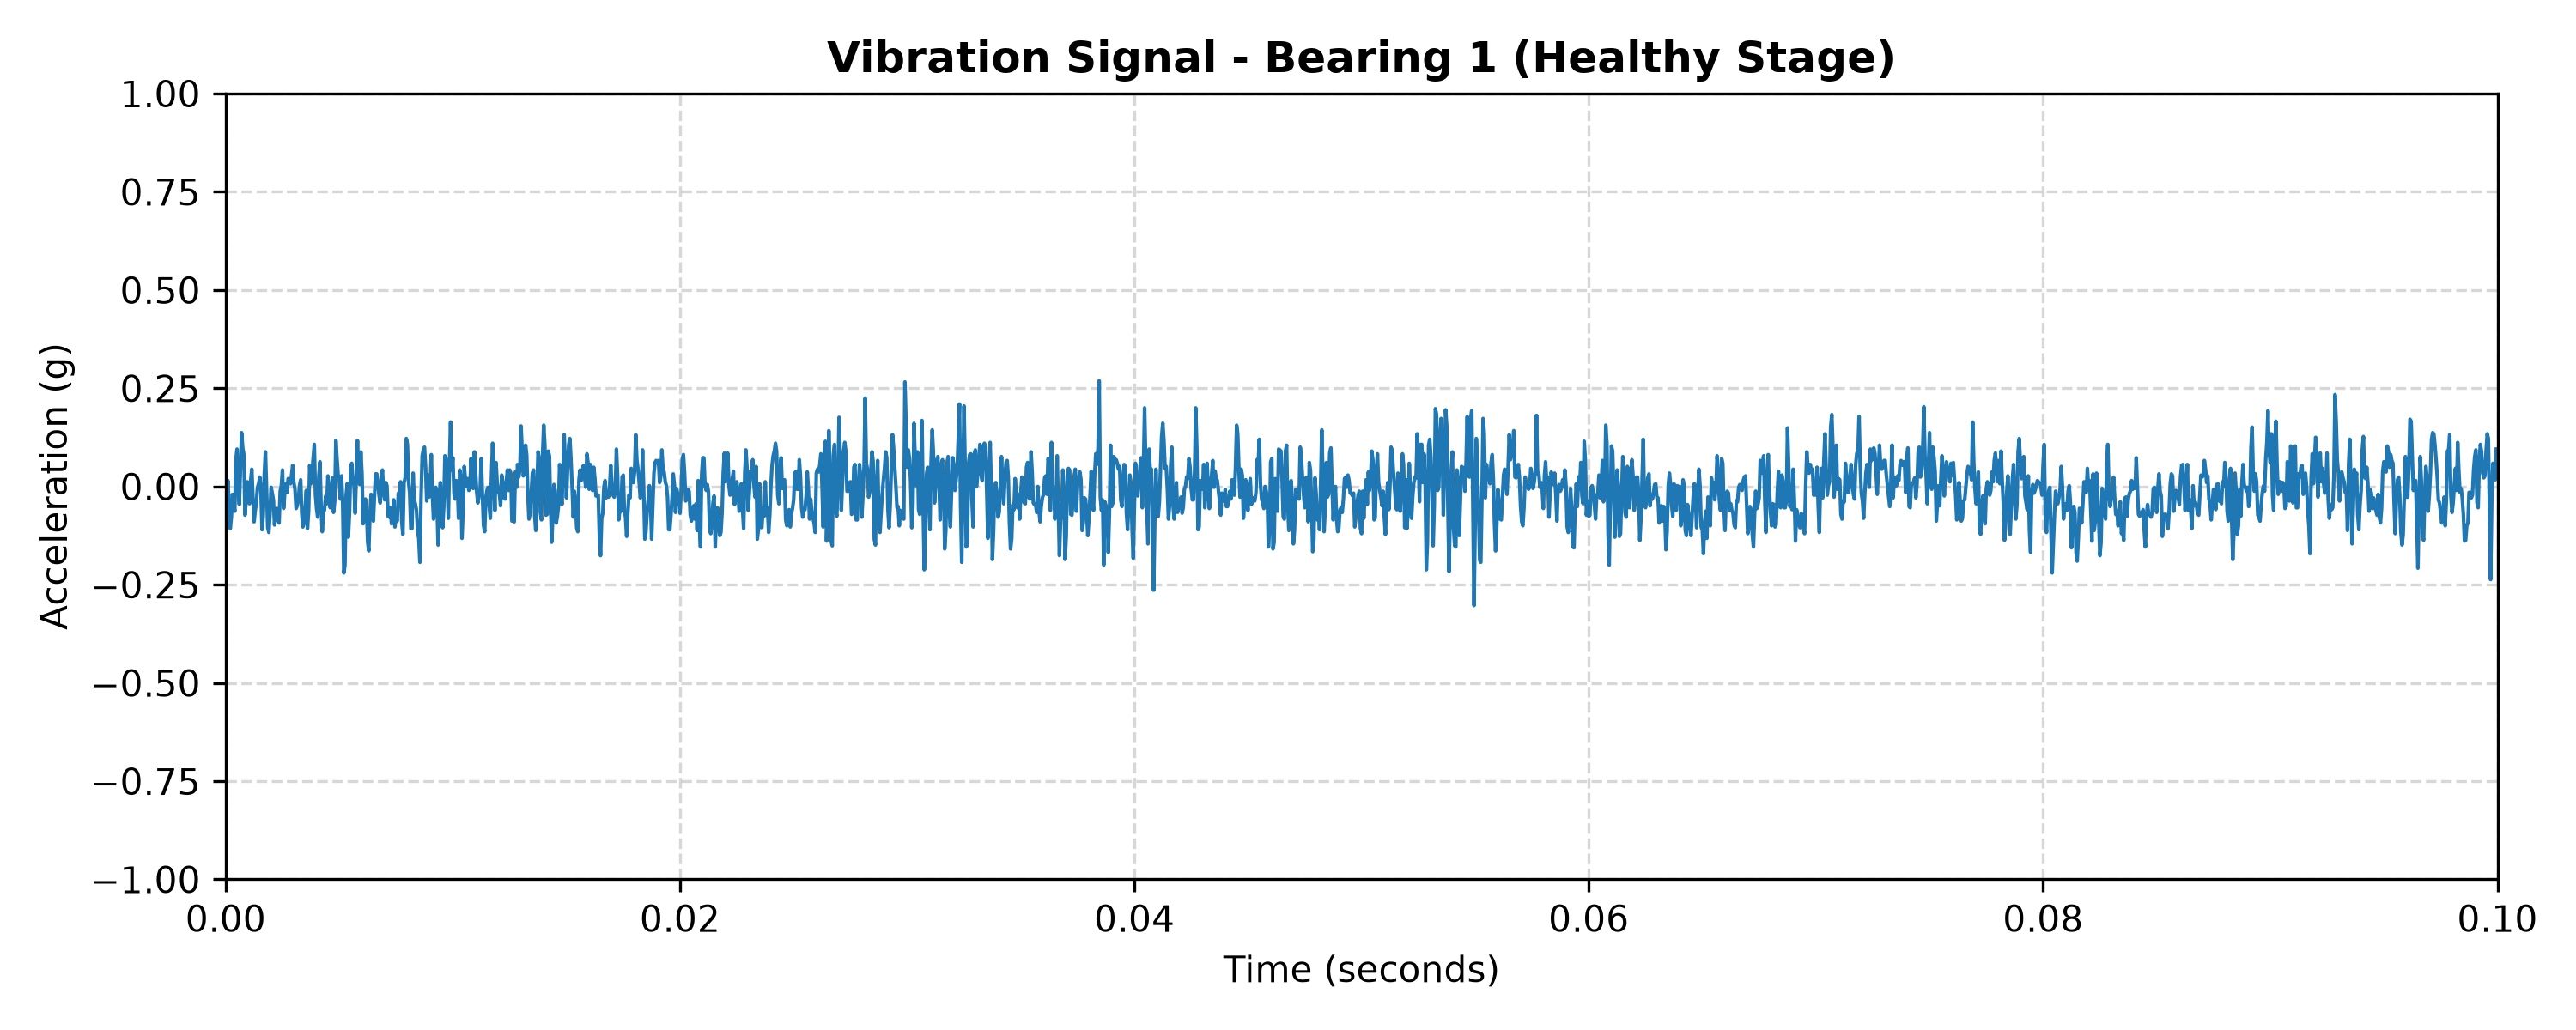
\includegraphics[width=0.95\textwidth]{raw_healthy_signal.png}
    \caption{Raw healthy signal segment from Bearing 1.}
    \label{fig:healthy_signal}
\end{figure}
\begin{figure}[htbp]
    \centering
    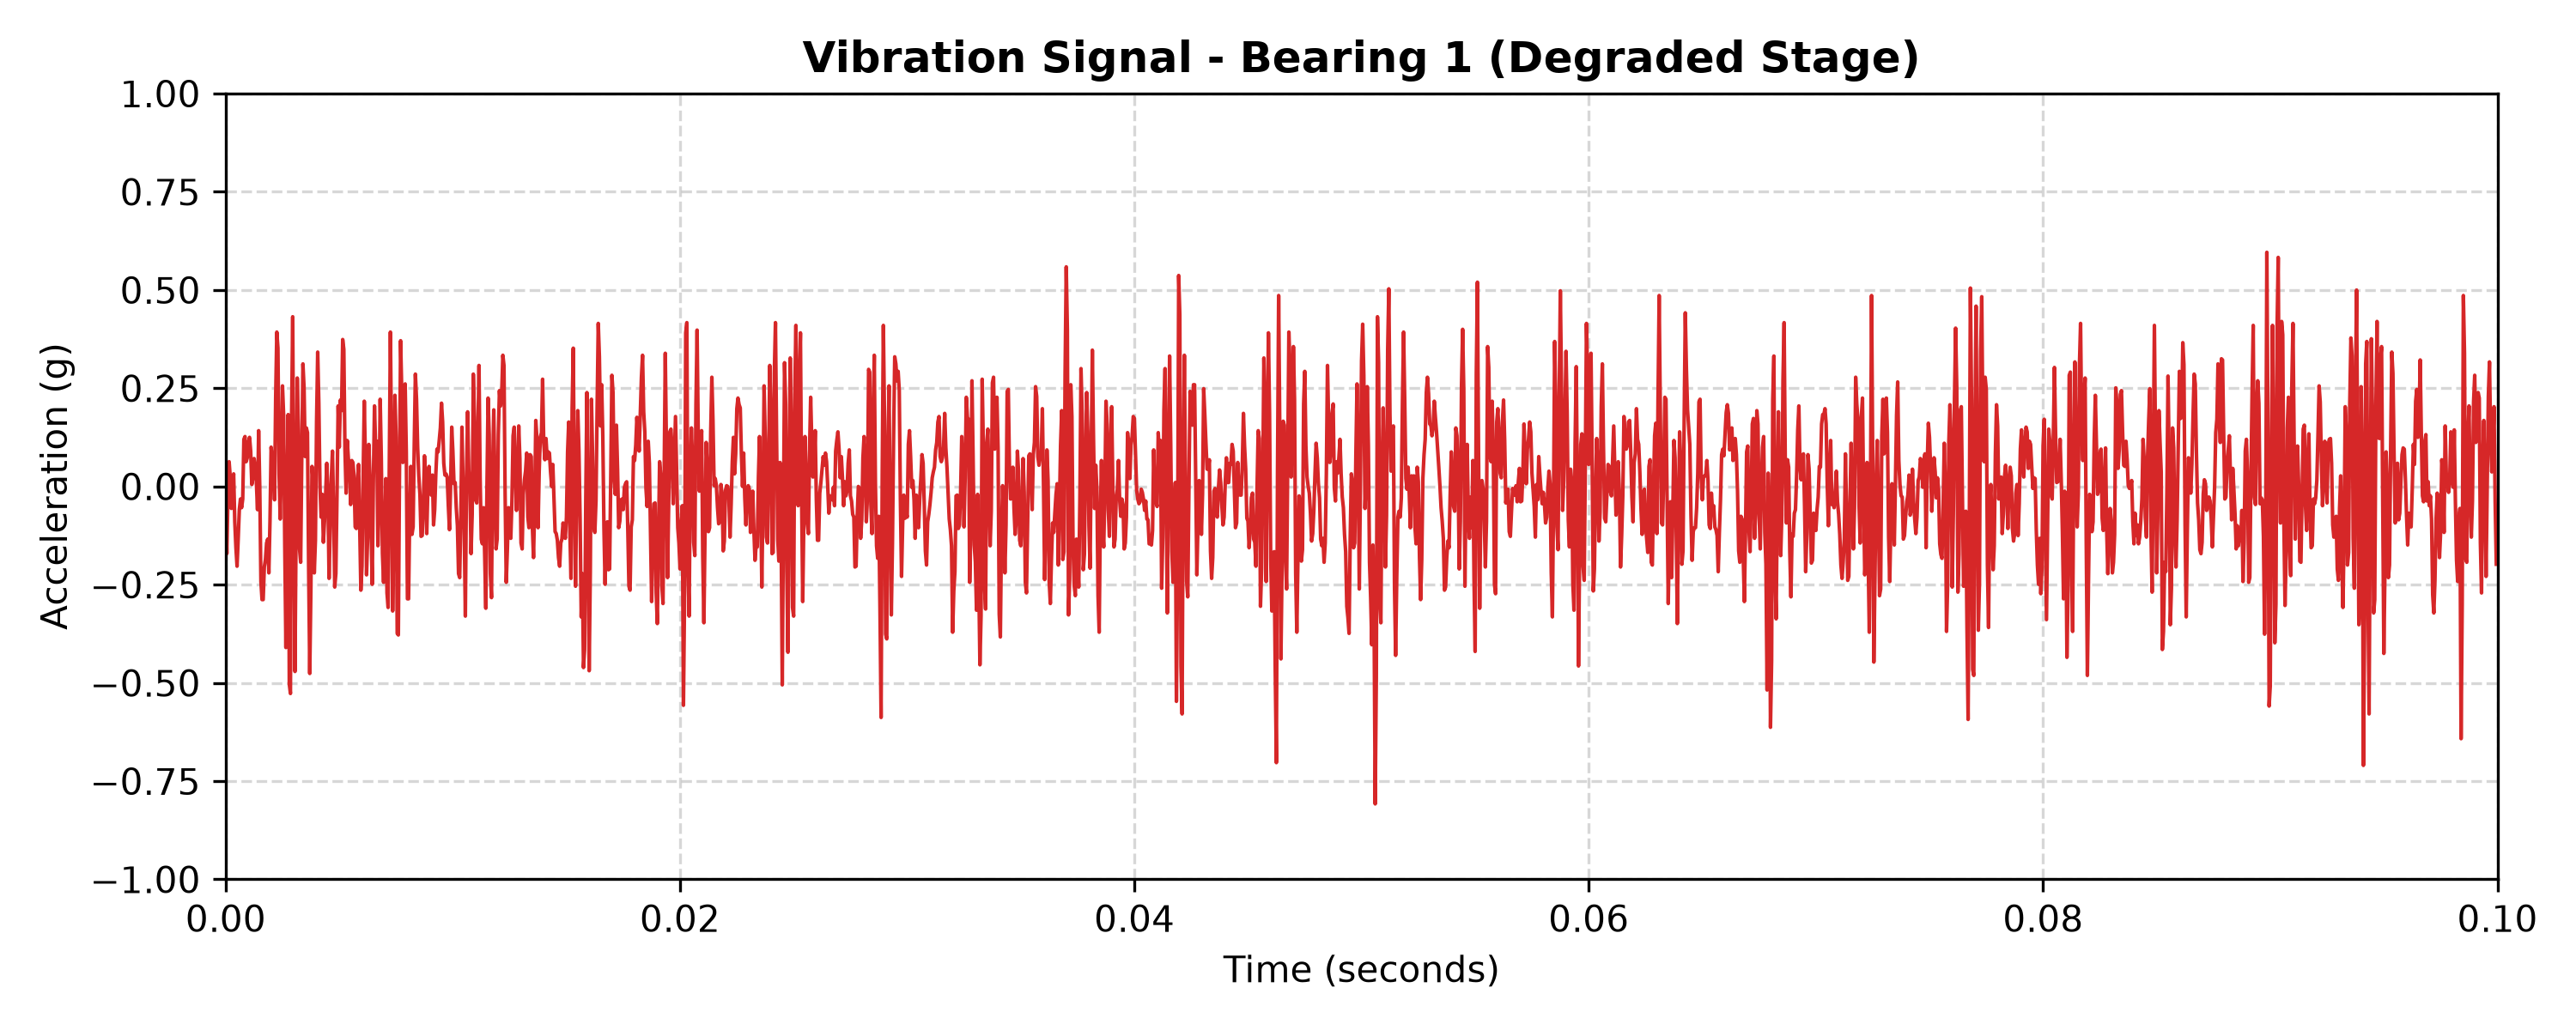
\includegraphics[width=0.95\textwidth]{raw_degraded_signal.png}
    \caption{Raw degraded signal segment from Bearing 1.}
    \label{fig:degraded_signal}
\end{figure}

\subsection{Signal segmentation}
Based on the initial exploratory analysis, the transition from a healthy state to early degradation and eventual failure was observed between February 15th and February 18th. To satisfy the Raspberry Pi memory and storage limitations constraints, a periodic sampling strategy was adopted. Only one out of every eight files ($step = 8$) was processed, yielding a sparse subset of $72$ independent records representing the vibration evolution every $\sim 80$ minutes.



Therefore, each $20.480$-sample record is segmented into smaller, non-overlapping time windows of $N = 2048$ samples, equivalent to $0.1$ seconds. A window of $0.1$ seconds is physically justified because the shaft rotates at $2000 \text{ RPM}$ ($\sim 33.3 \text{ Hz}$), meaning each segment captures approximately $3.3$ complete rotations. This length is perfectly sufficient to capture the periodic impact dynamics of localized bearing faults without inflating computational cost. A no overlap strategy is used between consecutive windows to minimize redundant computations, as the 10-minute gap between physical records already acts as a natural sparse sampling.

\subsection{Slope Entropy computation}
The Slope Entropy (SlpEn) algorithm is a non-linear time series complexity estimator based on symbolic patterns and amplitude information. The mathematical procedure follows these steps:
\begin{enumerate}
    \item \textbf{Normalization}: The input time series $x = \{x_0, x_1, \dots, x_{N-1}\}$ is first normalized using Z-score normalization ($y_i = \frac{x_i - \mu}{\sigma}$) to ensure the scale does not affect the thresholding process.
    \item \textbf{Subsequence Extraction}: Subsequences $y_m(j)$ of length $m$ (embedding dimension) are extracted starting from each index $j$.
    \item \textbf{Feature Extraction}: Given two consecutive samples $y_i$ and $y_{i-1}$ within the subsequence, thresholding rules based on parameters $\gamma$ and $\delta$ ($\gamma > \delta > 0$) map the differences to a symbol $s_i \in \{-2, -1, 0, 1, 2\}$:
    \begin{itemize}
        \item If $y_i > y_{i-1} + \gamma$, the symbol is $+2$.
        \item If $y_i > y_{i-1} + \delta$ and $y_i \le y_{i-1} + \gamma$, the symbol is $+1$.
        \item If $|y_i - y_{i-1}| \le \delta$, the symbol is $0$.
        \item If $y_i < y_{i-1} - \delta$ and $y_i \ge y_{i-1} - \gamma$, the symbol is $-1$.
        \item If $y_i < y_{i-1} - \gamma$, the symbol is $-2$.
    \end{itemize}
    \item \textbf{Pattern Identification}: Each subsequence of length $m$ yields a feature vector of $m-1$ symbols. We then count the occurrences of each unique pattern $k$.
    \item \textbf{Probability and Entropy}: The relative frequency of each unique pattern is computed as $p_k = \frac{c_k}{N - m + 1}$. Finally, the Shannon entropy is applied to these probabilities to compute the Slope Entropy:
    \begin{equation}
        SlpEn(m, \delta, \gamma) = - \sum_{k} p_k \ln(p_k)
    \end{equation}
\end{enumerate}

\subsection{Parameter selection}
The selection of parameters is critical to balance pattern richness with computational cost, particularly for embedded systems like the Raspberry Pi:
\begin{itemize}
    \item \textbf{Embedding Dimension ($m$)}: A value of $m=3$ is chosen. This yields feature vectors of length 2, resulting in $5^2 = 25$ possible unique patterns. This low dimensionality is ideal because it avoids the "curse of dimensionality", ensuring that the relative frequencies $p_k$ converge reliably even for short data segments ($N = 2048$). It also keeps memory requirements and computational overhead low on the Raspberry Pi.
    \item \textbf{Thresholds ($\gamma$ and $\delta$)}: Based on typical empirical recommendations for standardized vibration signals, we set $\gamma = 1.0$ and $\delta = 0.1$. The threshold $\gamma = 1.0$ standard deviation effectively captures the large impulsive transients generated by the bearing faults. The threshold $\delta = 0.1$ standard deviations serves as a noise filter, mapping negligible baseline fluctuations into the $0$ symbol, thereby increasing the algorithm's robustness against measurement noise.
\end{itemize}


\subsection{Experimental pipeline}
The overall pipeline for predictive maintenance consists of the following steps:
\begin{enumerate}
    \item \textbf{Data Acquisition \& Preprocessing}: Raw vibration signals are loaded, subsampled periodically (every $\sim 80$ minutes), and converted into a binary \texttt{.npz} format to optimize I/O on the RPi device.
    \item \textbf{Segmentation}: Each 1-second record is segmented into 10 sub-windows of 2048 samples.
    \item \textbf{Feature Extraction}: The optimized Slope Entropy algorithm is applied to each sub-window, and the average entropy for the record is computed to track temporal evolution.
    \item \textbf{Condition Monitoring \& Decision Making}: A statistical baseline is formed from the initial healthy records. A turning point (degradation onset) is flagged when the entropy deviates by more than 3 standard deviations from the baseline for at least 3 consecutive observations.
\end{enumerate}

\section{Experimental Setup}
All data processing and algorithmic evaluations were executed to run seamlessly on a realistic edge-computing node deployed in an industrial environment. The specific hardware employed was a Raspberry Pi 5 with 16GB of RAM, running the headless Raspberry Pi OS Lite (64-bit) to minimize background OS overhead. 

The edge device operated within a local area network (LAN), utilizing SSH (Secure Shell) for remote command execution. The raw sensor data acquired during the tests and the resulting output logs were securely transferred between the edge device using the SCP (Secure Copy Protocol).

\subsection{Implementation and optimization decisions}
Given the restrictive computational power and memory footprint typical of IoT systems, several critical software engineering decisions were made to optimize the predictive maintenance pipeline:
\begin{itemize}
    \item \textbf{Binary data conversion}: Raw vibration data was originally provided as thousands of uncompressed `.txt` files, causing massive I/O bottlenecks. These were periodically sampled (1 out of every 8 files) and serialized into a single, compressed binary \texttt{NumPy} archive (\texttt{.npz}). This reduced storage requirements and eliminated I/O latency during memory loading.
    \item \textbf{Complete vectorization}: The entire Slope Entropy algorithm was written relying exclusively on vectorized \texttt{NumPy} operations (implemented in backend C). Standard Python \texttt{for}-loops, which are  slow, were entirely avoided for the symbol-mapping and probability-counting phases.
    \item \textbf{Low embedding dimension}: An embedding dimension of $m=3$ was deliberately chosen. This capped the possible unique symbolic patterns to $5^2 = 25$, avoiding the combinatorial explosion that would otherwise exponentially consume RAM and CPU cycles for pattern matching.
\end{itemize}


\section{Results}
The temporal evolution of the Slope Entropy over the 72 processed records is presented in Figure \ref{fig:entropy_evolution}. 

\begin{figure}[htbp]
    \centering
    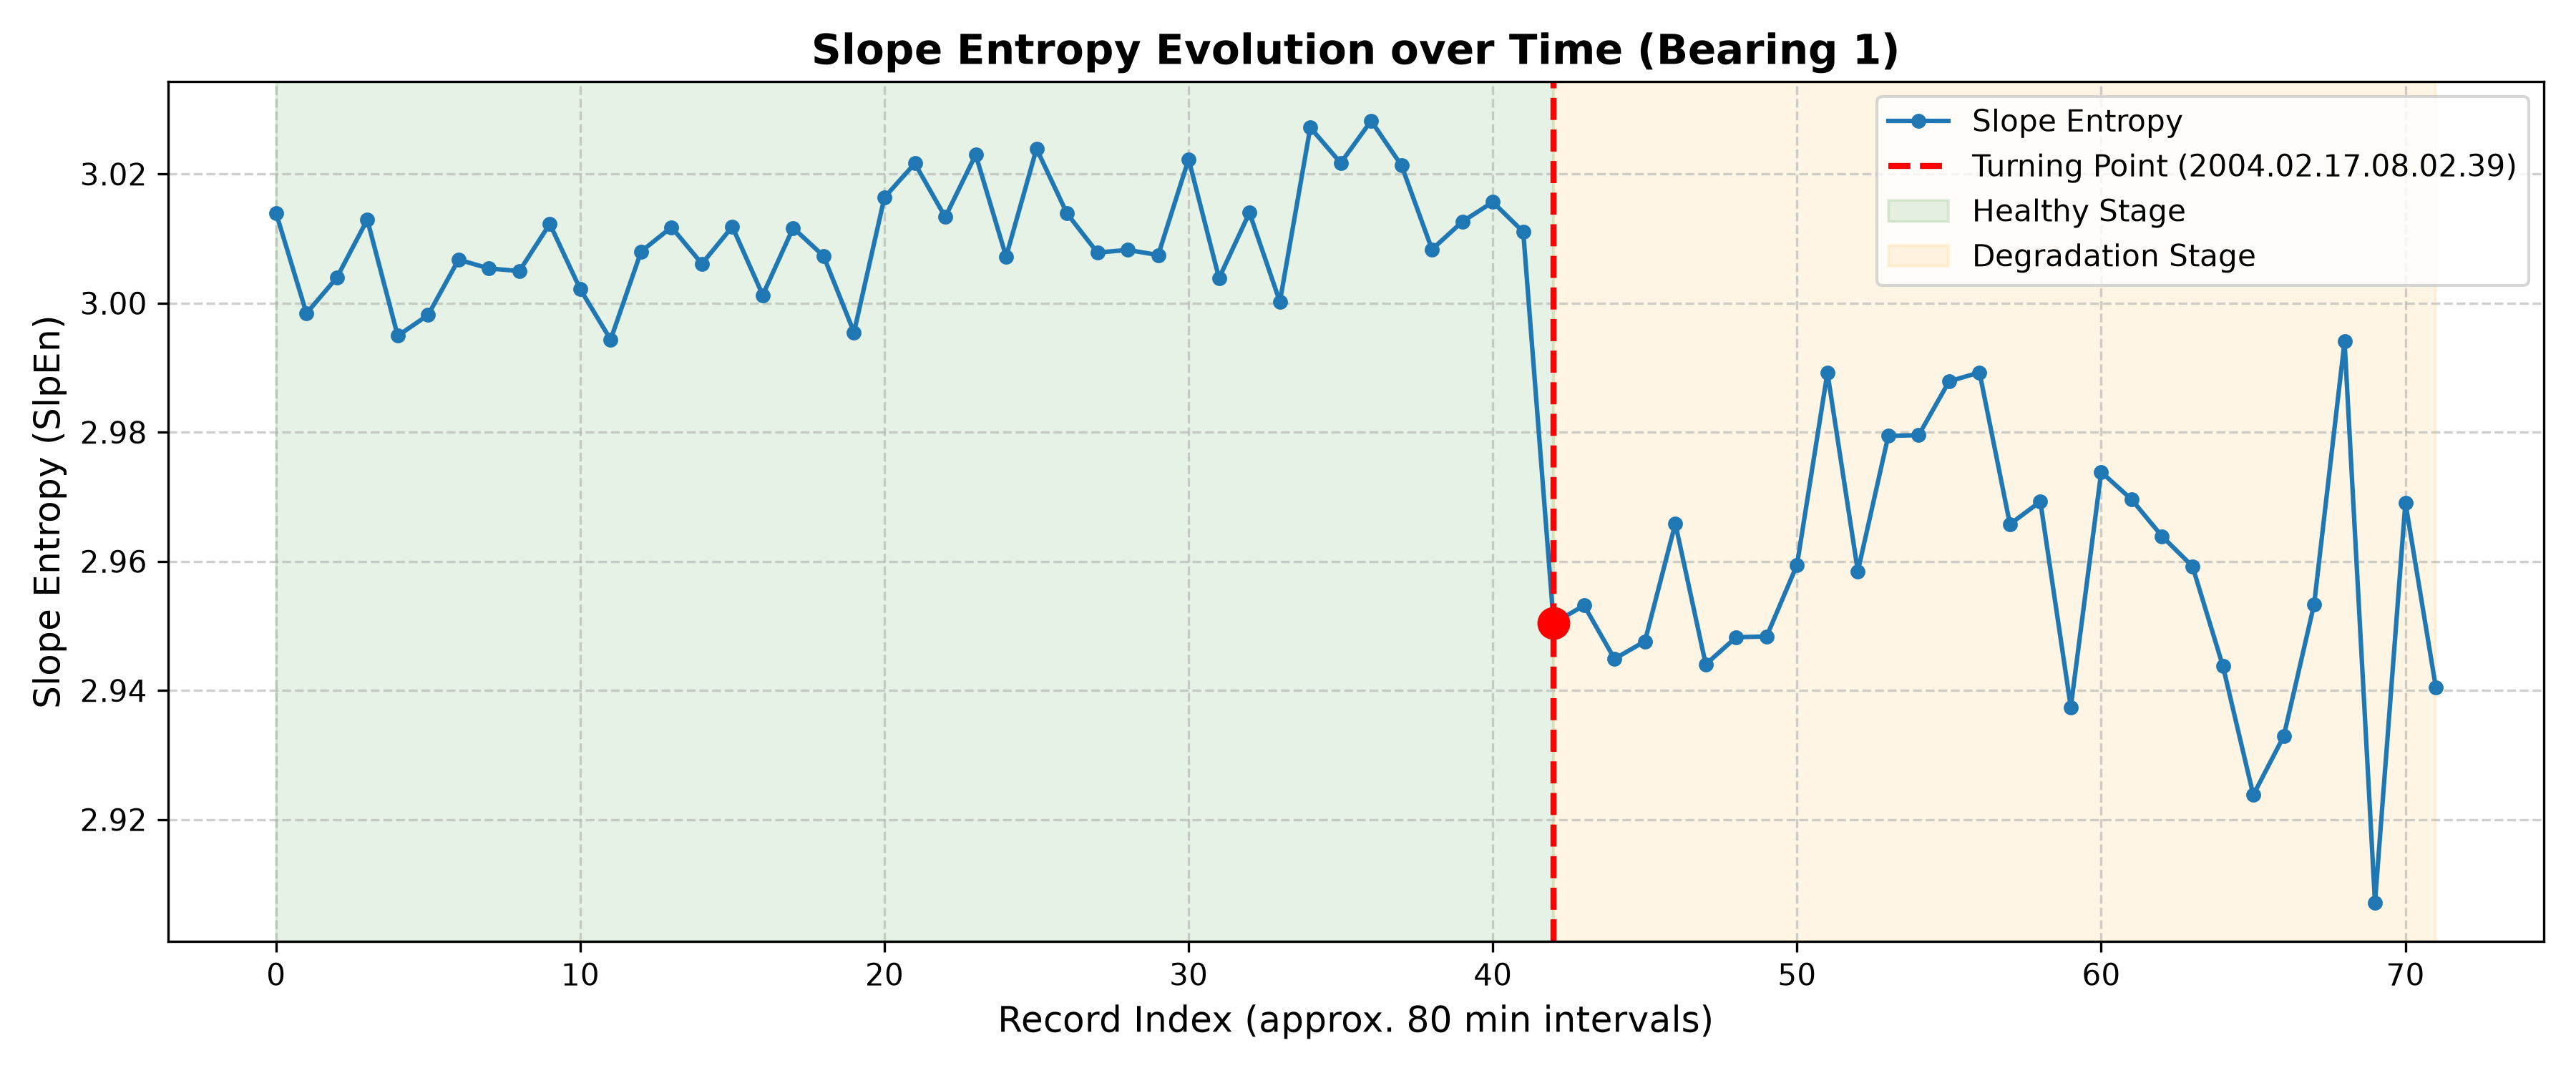
\includegraphics[width=0.95\textwidth]{entropy_evolution.png}
    \caption{Temporal evolution of Slope Entropy for Bearing 1. The turning point marks the transition from healthy operation to progressive degradation.}
    \label{fig:entropy_evolution}
\end{figure}

During the initial stage (records 0 to 41), the Slope Entropy maintains a relatively high and stable value ($\approx 3.01$), indicating the highly complex and somewhat random nature of the healthy bearing vibrations. However, at record 42 (Timestamp: \texttt{2004.02.17.08.02.39}), the automatic detection criterion flagged a significant and sustained drop in entropy.

\subsection{Comparative analysis}
To thoroughly evaluate the effectiveness of the algorithm, a comparative analysis was performed across the three distinct operational states: Healthy, Transition (turning point), and Faulty (late degradation). Both classical linear metrics and the non-linear Slope Entropy were calculated.

\textbf{Quantitative Comparison:}
Table \ref{tab:comparison} summarizes the statistical and entropic features for representative records of each stage.

\begin{table}[htbp]
    \centering
    \begin{tabularx}{\textwidth}{X c S S S S}
    \toprule
    \textbf{Operational Stage} & \textbf{Timestamp} & \textbf{RMS (g)} & \textbf{P2P (g)} & \textbf{Kurtosis} & \textbf{SlpEn} \\
    \midrule
    Healthy & 2004.02.15.00.02.39 & 0.078 & 0.717 & 3.37 & 3.014 \\
    Transition & 2004.02.17.08.02.39 & 0.172 & 1.760 & 5.62 & 2.950 \\
    Faulty & 2004.02.18.22.42.39 & 0.197 & 1.865 & 4.43 & 2.941 \\
    \bottomrule
    \end{tabularx}
    \caption{Quantitative comparison of bearing vibration features across degradation stages.}
    \label{tab:comparison}
\end{table}

\textbf{Qualitative Comparison:}
\begin{itemize}
    \item \textbf{Healthy Stage}: The vibration signal is characterized by low amplitude (RMS $\approx 0.078$ g) and a kurtosis close to 3. The high Slope Entropy ($3.014$) confirms that the signal is dominated by unpredictable, random friction noise with high structural complexity.
    \item \textbf{Transition Stage}: At the onset of degradation (turning point), a tiny defect appears on the outer race. While RMS and P2P double, the most significant change is the sharp spike in Kurtosis ($5.62$), reflecting the sporadic, high-energy impulsive shocks. Slope Entropy begins to drop ($2.950$) as the periodic nature of the impacts introduces deterministic patterns into the signal.
    \item \textbf{Faulty Stage}: In advanced degradation, the damage propagates across the bearing. The RMS and Peak-to-Peak values reach their maximums, indicating severe, continuous impacts. Interestingly, the Kurtosis drops ($4.43$) compared to the transition stage because the impacts are no longer isolated rare events, but rather a constant feature of the baseline signal. Slope Entropy reaches its lowest point ($2.941$), confirming that the dynamic system behavior is now highly deterministic and structured by the rotational frequency hitting the severe fault.
\end{itemize}

\subsection{Parameter sensitivity analysis}
The robustness of the Slope Entropy algorithm was evaluated by varying the primary amplitude threshold parameter $\gamma \in \{0.5, 1.0, 1.5\}$ while holding the embedding dimension ($m=3$) and the noise filter threshold ($\delta=0.1$) constant. The goal is to determine if the turning point remains detectable regardless of minor tuning variations.

\begin{figure}[htbp]
    \centering
    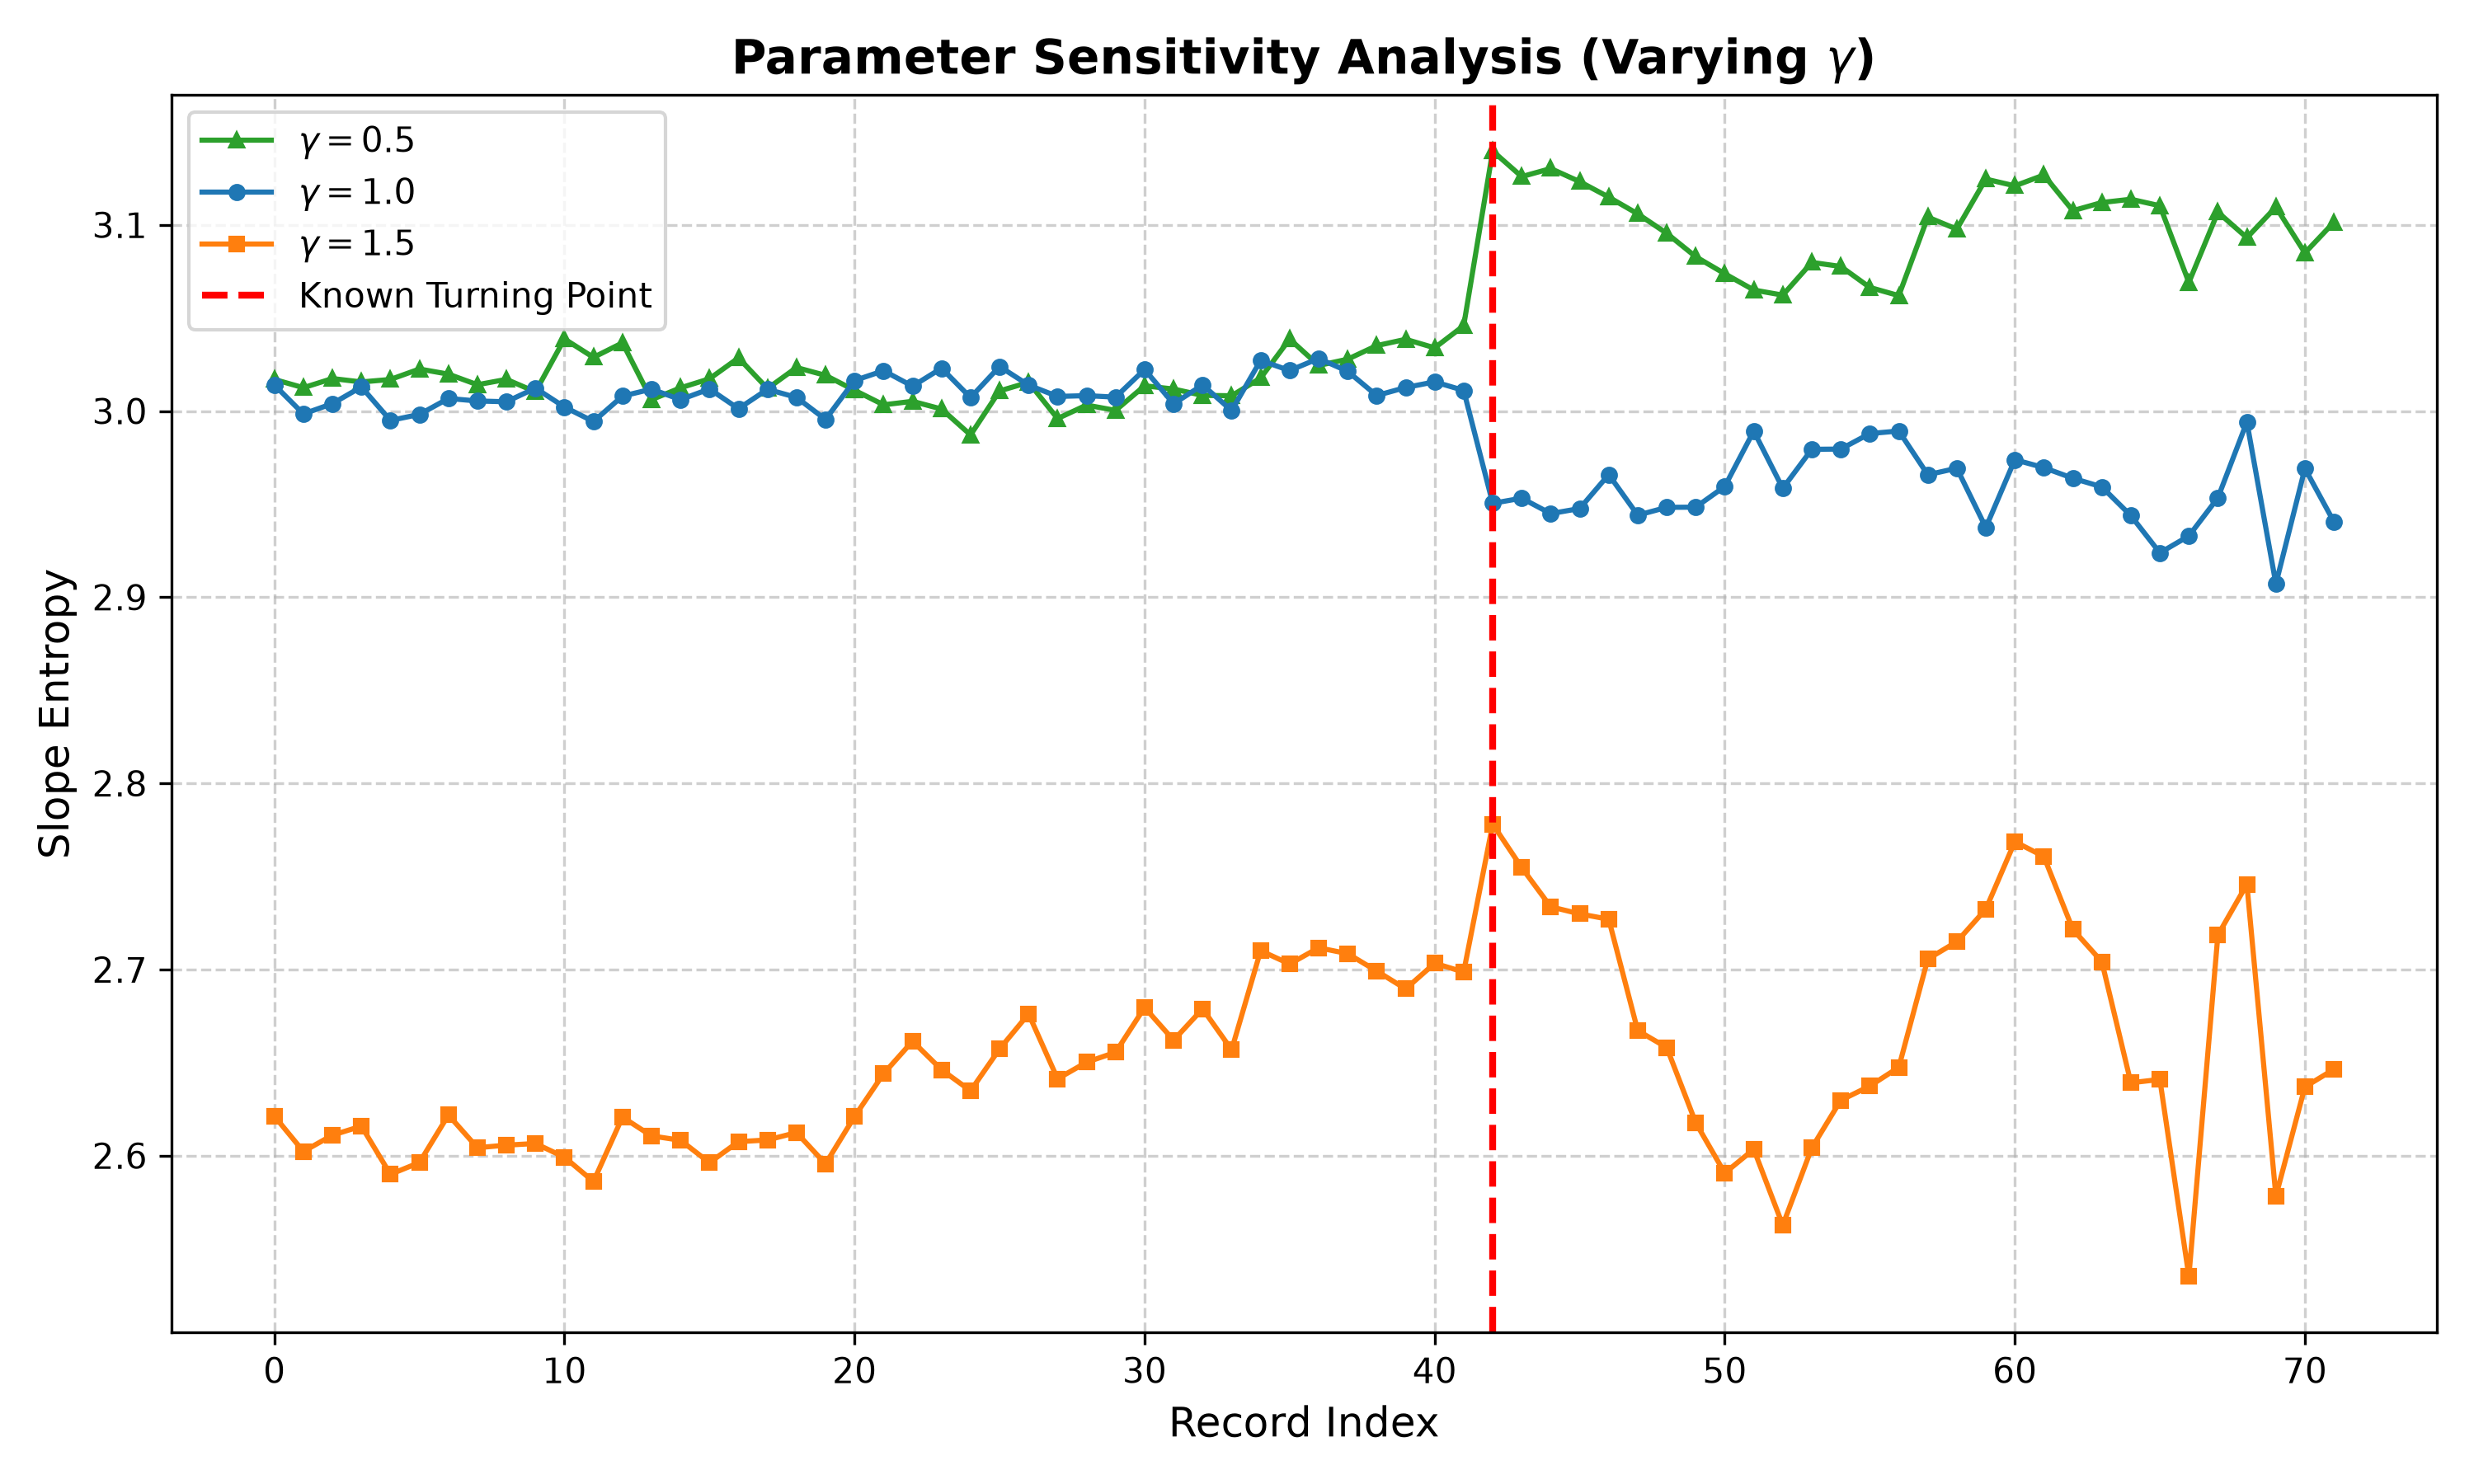
\includegraphics[width=0.95\textwidth]{parameter_sensitivity.png}
    \caption{Sensitivity analysis of the Slope Entropy algorithm under different $\gamma$ thresholds.}
    \label{fig:parameter_sensitivity}
\end{figure}

As shown in Figure \ref{fig:parameter_sensitivity}, while the absolute values of the Slope Entropy shift vertically depending on the strictness of the $\gamma$ threshold (tighter thresholds yield slightly higher base entropies because more differences are classified as random noise rather than distinct symbols), the overall temporal trend remains practically identical. The sharp drop indicating the turning point at record 42 is distinctly visible in all three configurations. This proves that the proposed method is highly robust and not overly sensitive to precise parameter fine-tuning, which is highly advantageous for automated deployment in industrial systems.

\subsection{Computational cost and feasibility}
To evaluate the feasibility of deploying the proposed pipeline in a real-time industrial edge computing environment, execution time metrics were profiled for each stage of the process.

\begin{figure}[htbp]
    \centering
    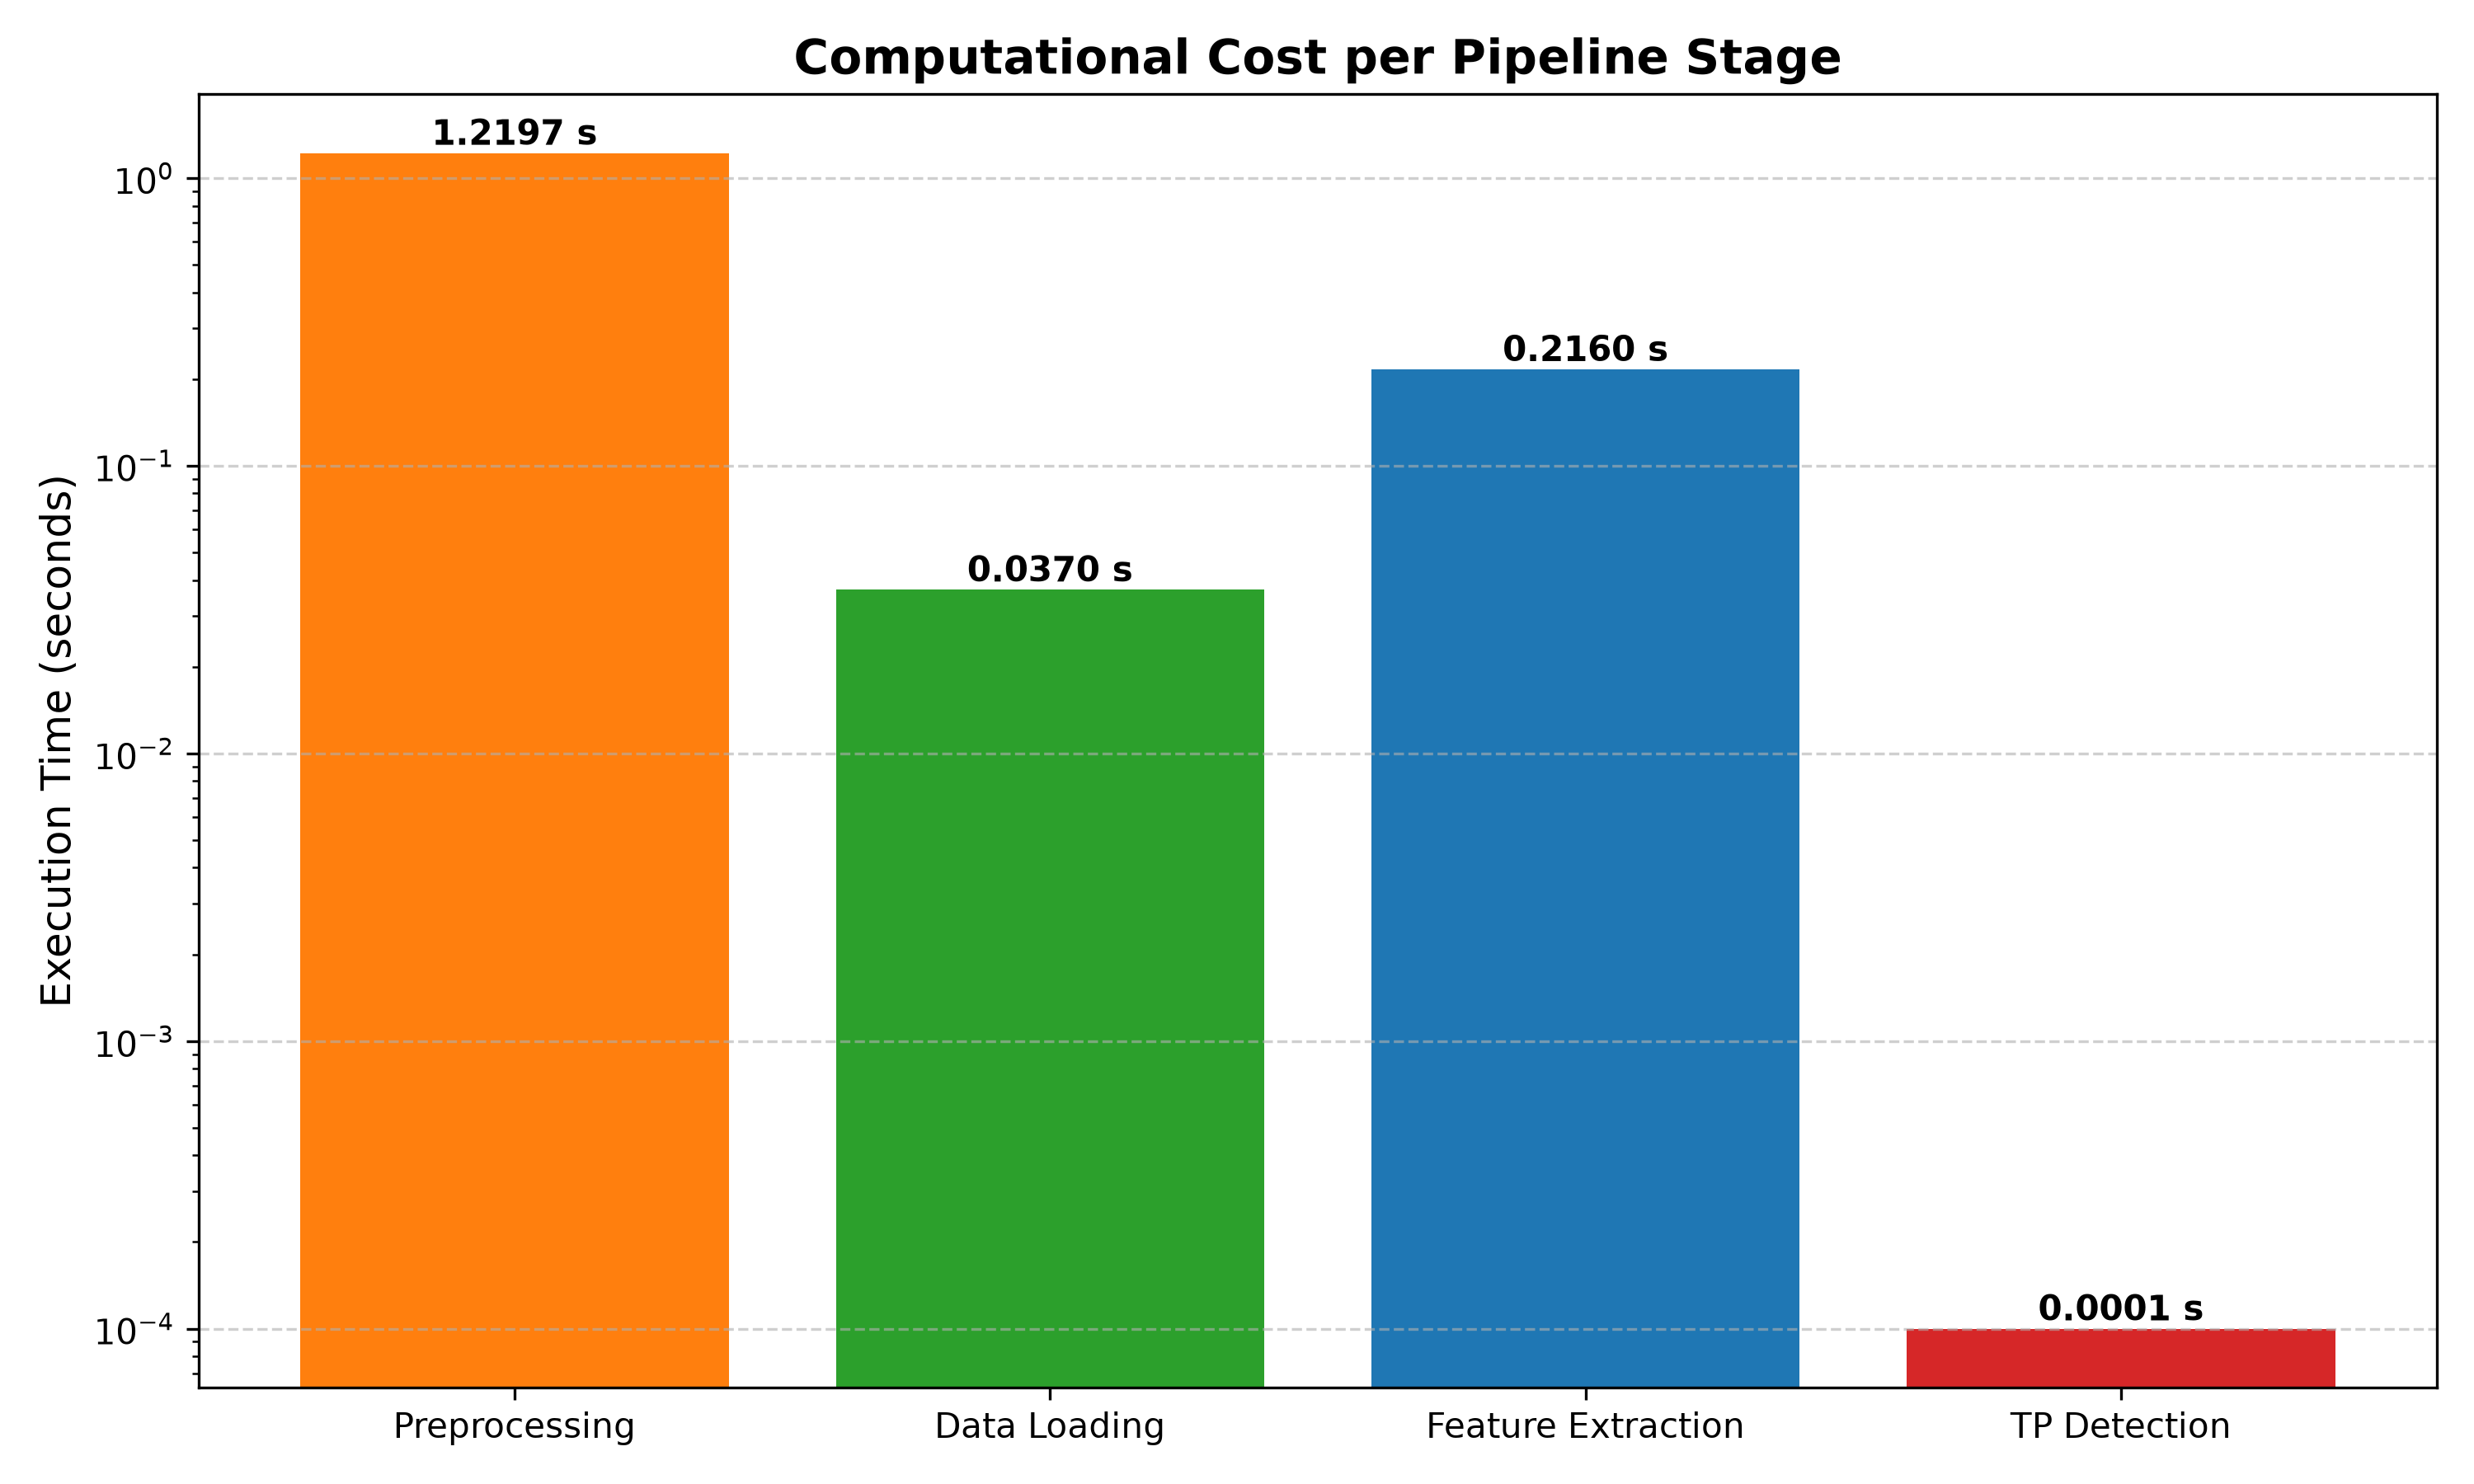
\includegraphics[width=0.85\textwidth]{computational_cost.png}
    \caption{Computational cost (execution time) per pipeline stage, plotted on a logarithmic scale.}
    \label{fig:computational_cost}
\end{figure}

As shown in Figure \ref{fig:computational_cost}, the computational bottleneck resides entirely in the Data Preprocessing stage ($\approx 1.219$ s), which involves reading thousands of text files and compressing them into a binary format. However, in a real-world edge deployment, this step is bypassed as the sensor data is fed directly into memory arrays.

The core of the condition monitoring algorithm, the Feature Extraction using Slope Entropy exhibits extreme efficiency. Calculating the entropy for all 72 records (comprising over 147,000 samples) took  $\approx 0.216$ seconds. Furthermore, the statistical Turning Point Detection was instantaneous ($\approx 0.001$ s). This outstanding performance confirms that the vectorized, low-embedding-dimension ($m=3$) Slope Entropy algorithm is computationally trivial and highly feasible for real-time fault detection on resource-constrained embedded systems.

\section{Discussion}
The turning point detected on February 17th aligns perfectly with the physical degradation of the bearing. As the outer race defect emerged and grew, the vibration signal transitioned from random noise (high complexity) to a more deterministic, periodic series of impulsive impacts (lower complexity). Slope Entropy successfully captured this dynamic shift long before the catastrophic failure occurred on February 19th.

The algorithmic and computational evaluations confirm that this non-linear approach is not only mathematically robust against interference but also highly viable for edge computing on restrictive IoT platforms.

\section{Conclusion}
This study successfully demonstrates the application of Slope Entropy for early fault detection in industrial bearings under embedded-system constraints. The proposed pipeline accurately detected the onset of degradation well in advance of the final failure, highlighting the potential of non-linear time series analysis for predictive maintenance. Future work could explore adaptive thresholding to further improve robustness across different machine operating conditions.

\begin{thebibliography}{9}

\bibitem{qiu2006wavelet}
Hai Qiu, Jay Lee, Jing Lin, and Gang Yu.
\newblock Wavelet filter-based weak signature detection method and its application on rolling element bearing prognostics.
\newblock \emph{Journal of Sound and Vibration}, 289:1066--1090, 2006.

\bibitem{frosini2015induction}
Lucia Frosini, Ciprian Harli{\c{s}}ca, and Lor{\'a}nd Szab{\'o}.
\newblock Induction Machine Bearing Fault Detection by Means of Statistical Processing of the Stray Flux Measurement.
\newblock \emph{IEEE Transactions on Industrial Electronics}, 62(3):1846--1854, 2015.

\bibitem{jiang2016hidden}
Huiming Jiang, Jin Chen, and Guangming Dong.
\newblock Hidden Markov model and nuisance attribute projection based bearing performance degradation assessment.
\newblock \emph{Mechanical Systems and Signal Processing}, 72-73:184--205, 2016.

\bibitem{gao2017multi}
Yangde Gao, Francesco Villecco, Ming Li, and Wanqing Song.
\newblock Multi-Scale Permutation Entropy Based on Improved LMD and HMM for Rolling Bearing Diagnosis.
\newblock \emph{Entropy}, 19(176), 2017.

\bibitem{cuesta2019slope}
David Cuesta-Frau.
\newblock Slope Entropy: A New Time Series Complexity Estimator Based on Both Symbolic Patterns and Amplitude Information.
\newblock \emph{Entropy}, 21(1167), 2019.

\end{thebibliography}

\end{document}
